\begin{frame}
  \frametitle{Некоторые определения из теории абсолютно твердого тела}
  
  \emph{Неизменяемая система} — система материальных точек, в которой расстояние между двумя любыми точками постоянно. При непрерывном распределении масс такая система идеальный образ твердого тела и называется \emph{абсолютно твердым телом}~\cite[48]{Buhgoltz1965}.

  Различают абсолютно твердые тела:
  \begin{itemize}
    \item с одной неподвижной точкой,
    \item свободные.
  \end{itemize}
  
  \begin{block}{Теорема Эйлера}
    всякое перемещение абсолютно твердого тела около неподвижной точки можно получить одним только поворотом тела вокруг определенной оси, проходящей через эту точку и называемой осью конечного вращения~\cite[132]{Buhgoltz1965}.
  \end{block}

  \begin{block}{Теорема Шаля}
    всякое перемещение свободного абсолютно твердого тела из одного положения в другое может быть получено посредством поступательного перемещения вместе с произвольно выбранным полюсом и поворота вокруг некоторой оси, проходящей через этот полюс~\cite[153]{Buhgoltz1965}.
  \end{block}
  Мишель Шаль, 1793--1880 гг. — французский геометр.
\end{frame}

%%----------------------------------------------------------
\begin{frame}
  \frametitle{Винтовое движение}
  \begin{block}{Теорема Шаля (другая формулировка)}
    всякое перемещение свободного абсолютно твердого тела может быть осуществлено одним винтовым движением около некоторой винтовой оси, называемой осью конечного винтового перемещения.
  \end{block}

  Пусть движение тела слагается из:
  \begin{itemize}
    \item равномерного вращения вокруг оси постоянного направления с угловой скоростью $\vb{\omega}$;
    \item равномерного прямолинейного поступательного движения с постоянной скоростью $\vb{v}$, параллельной $\vb{\omega}$.
  \end{itemize}
  Результирующее движение тела в этом случае называется \emph{винтовым движением}, а ось вращения — \emph{осью винта}~\cite[146]{Buhgoltz1965}. Любая точка тела остается во время винтового движения на поверхности круглого цилиндра, описывая винтовую линию.
\end{frame}

%%----------------------------------------------------------
\begin{frame}
  \frametitle{Принцип перенесения Котельникова--Штуди}
  \begin{block}{Принцип перенесения}
    Все формулы теории конечных поворотов и кинематики движения твердого тела с одной неподвижной точкой при замене в них вещественных величин на дуальные аналоги переходят в формулы теории конечных перемещений и кинематики движения свободного твердого тела~\cite[67]{Chelnokov:2006}.
  \end{block}
  Иначе говоря, если в формулах для вращения точки в пространстве заменить вещественные числа, векторы, углы и кватернионы на дуальные числа, винты, дуальные углы и бикватернионы, то получатся корректные формулы для винтового движения.
  Принцип сформулирован Котельниковым Александр Петровичем и Эдуардом Штуди (Eduard Study)~\cite[12--13]{Dimentberg:1965}.

  \begin{center}
    \begin{tblr}{hlines = {0.5pt,solid}, vlines = {red3,dashed}}
      Радиус вектор $\vb{p}$ & Винт $\vb{L}$\\
      Угол $\theta$ & Дуальный угол $\Theta$\\
      Действительное число $\lambda$ & Дуальное число $\Lambda$\\
    \end{tblr}
  \end{center}

  Если формулы для вращений в пространстве применяются к \textbf{аффинным точкам} (радиус векторам), то полученные по принципу перенесения формулы следует применять к \textbf{винтам} то есть к \textbf{прямым} в пространстве.
\end{frame}

%%----------------------------------------------------------
\begin{frame}
  \frametitle{Винтовое движение прямой}
  \begin{columns}
    \begin{column}{0.4\textwidth}
      \begin{center}
        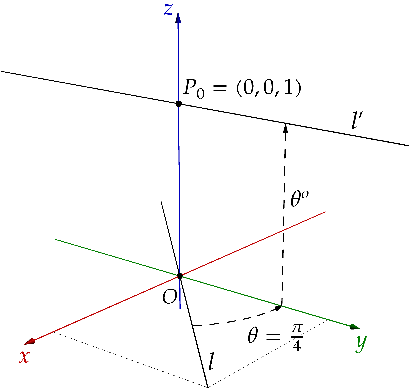
\includegraphics[width=\textwidth]{img/screws/moment07}
      \end{center}
    \end{column}
    \begin{column}{0.6\textwidth}
      Рассмотрим прямую $l$ лежащую в плоскости $Oxy$ с направляющим вектором $\vb{v} = (1, 1, 0)^T$, проходящую через точку $O$. Зная $\vb{p} = (0, 0, 0)^T$ и направляющий вектор $\vb{v}$ вычислим момент прямой:
      \begin{equation*}
        \vb{m} = \vb{p} \times \vb{v} = \vb{0},
      \end{equation*}
      что дает представление прямой в виде мотора
      \begin{equation*}
        \vb{L} = \vb{v} + \vb{0}\varepsilon.
      \end{equation*}
      Подвергнем $l$ винтовому движению вдоль оси $Oz$ повернув на $\pi/4$ и подняв на $1$ вверх по оси. Для этого зададим дуальный угол
      \begin{equation*}
        \Theta = \pi/4 + \varepsilon
      \end{equation*}
      и подставим его в матрицу элементарного поворота вокруг оси $Oz$:
      \begin{equation*}
        R_{z}(\Theta) = 
        \begin{bmatrix}
          \cos\Theta & -\sin\Theta & 0\\
          \sin\Theta & \cos\Theta & 0\\
          0 & 0 & 1
        \end{bmatrix}
      \end{equation*}
    \end{column}
  \end{columns}
\end{frame}

%%----------------------------------------------------------
\begin{frame}
  \frametitle{Винтовое движение прямой}
  \begin{columns}
    \begin{column}{0.4\textwidth}
      \begin{center}
        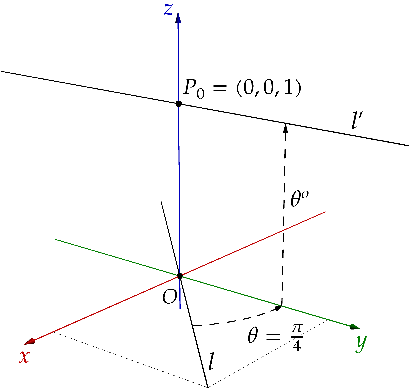
\includegraphics[width=\textwidth]{img/screws/moment07}
      \end{center}
    \end{column}
    \begin{column}{0.6\textwidth}
      Матрица $R_{z}(\Theta)$ — матрица с дуальными коэффициентами. Умножим ее на винт, представив последний как вектор с дуальными коэффициентами:
      \begin{equation*}
        \vb{L}^\prime = R_z(\Theta) \vb{L} = 
        \begin{bmatrix}
          \cos\Theta & -\sin\Theta & 0\\
          \sin\Theta & \cos\Theta & 0\\
          0 & 0 & 1
        \end{bmatrix}
        \begin{bmatrix}
          1\\1\\0
        \end{bmatrix}
        =
        \begin{bmatrix}
          \cos\Theta - \sin\Theta\\
          \cos\Theta + \sin\Theta\\
          0
        \end{bmatrix}
      \end{equation*}
      Так как $\Theta = \theta + \theta^o \varepsilon$, то
      \begin{align*}
        & \cos\Theta - \sin\Theta = \cos\theta - \sin\theta - (\cos\theta + \sin\theta)\theta^o\varepsilon,\\
        & \cos\Theta + \sin\Theta = \cos\theta +\sin\theta + (\cos\theta - \sin\theta)\theta^o\varepsilon.
      \end{align*}
      Подставим $\Theta = \pi/4 + 1$ и получим:
      \begin{equation*}
        \cos\Theta - \sin\Theta = -\sqrt{2}\varepsilon,
        \quad
        \cos\Theta + \sin\Theta = +\sqrt{2}.
      \end{equation*}
      \begin{equation*}
        \vb{L}^{\prime} =
        \begin{bmatrix}
          -\sqrt{2}\varepsilon\\
          \sqrt{2}\\
          0  
        \end{bmatrix}
        =
        \begin{bmatrix}
          0\\ \sqrt{2} \\ 0
        \end{bmatrix}
        +
        \varepsilon
        \begin{bmatrix}
          -\sqrt{2}\\
          0\\
          0
        \end{bmatrix}
      \end{equation*}
    \end{column}
  \end{columns}
\end{frame}

%%----------------------------------------------------------
\begin{frame}
  \frametitle{Винтовое движение прямой}
  \begin{columns}
    \begin{column}{0.4\textwidth}
      \begin{center}
        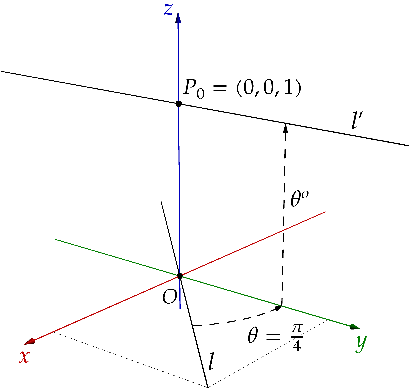
\includegraphics[width=\textwidth]{img/screws/moment07}
      \end{center}
    \end{column}
    \begin{column}{0.6\textwidth}
      Нормируем винт $\vb{L}^{\prime}$ поделив и векторную и моментную части на норму $\norm{\vb{L}^{\prime}}$. Так как выполняется условие Плюккера:
      \begin{equation*}
        (\vb{v}^{\prime}, \vb{m}^{\prime}) = 0 \cdot (-\sqrt{2}) + \sqrt{2} \cdot 0 + 0\cdot 0 = 0,
      \end{equation*}
      то винт задает прямую и его норма — действительное число $\norm{\vb{L}^{\prime}} = \sqrt{2}$.
      \begin{equation*}
        \hat{\vb{L}}^{\prime} = \hat{\vb{v}}^{\prime} + \hat{\vb{m}}^{\prime}\varepsilon = (0, 1, 0)^T + \varepsilon (-1, 0, 0)^T.
      \end{equation*}
      Найдем точку прямой, вычислив координаты проекции начала координат на прямую:
      \begin{equation*}
        \vb{p}^{\prime}_{0} = 
        \dfrac{\hat{\vb{v}}^{\prime} \times \hat{\vb{m}}^{\prime}}{\norm{\hat{\vb{v}}^{\prime}}^2} = 
        \begin{vmatrix}
          \vb{i} & \vb{j} & \vb{k}\\
          1 & 0 & 0\\
          0 & 1 & 0
        \end{vmatrix}
        =
        \begin{bmatrix}
          0\\0\\+1
        \end{bmatrix}
      \end{equation*}
      Таким образом винт $\hat{\vb{L}}^{\prime}$ задает прямую, проходящую через точку $P_0 = (0, 0, 1)$ по направлению $\hat{\vb{v}}^{\prime} = (0, 1, 0)^T$. 
    \end{column}
  \end{columns}
\end{frame}

%%----------------------------------------------------------
\begin{frame}
  \frametitle{Получение винтового аналога формулы Родрига с коэффициентами Родрига--Гамильтона}
  Для вращения точки $P$ с радиус вектором $\vb{p}=(x, y, z)^T$ абсолютно твердого тела с закрепленной точкой, вокруг оси, проходящей через начало координат с направляющим вектором $\vb{a}=(a_x, a_y, a_z)^T$ справедлива следующая формула:
  \begin{equation*}
    \vb{p}^{\prime} = \vb{p} +2\lambda_0 \vb{\lambda} \times \vb{p} + 2\vb{\lambda}\times\vb{\lambda}\times\vb{p},
  \end{equation*}
  где $\lambda_0$, $\vb{\lambda} = (\lambda_1, \lambda_2, \lambda_3)^T$ --- коэффициенты Родрига--Гамильтона, которые вычисляются как
  \begin{equation*}
    \lambda_0 = \cos\dfrac{\theta}{2},\;
    \vb{\lambda} = \sin\dfrac{\theta}{2}\vb{a}\; \Leftrightarrow\;
    \lambda_1 = \sin\dfrac{\theta}{2}a_x,\;
    \lambda_2 = \sin\dfrac{\theta}{2}a_y,\;
    \lambda_3 = \sin\dfrac{\theta}{2}a_z,
  \end{equation*}
  где $\theta$ --- величина угла поворота вокруг оси с направляющим вектором $\vb{a}$.

  Согласно принципу перенесения следует сделать следующие замены:
  \begin{center}
    \begin{tblr}{hlines = {0.5pt,solid}, vlines = {red3,dashed}}
      Вращение & Винтовое движение\\
      $\vb{p} = (x, y, z)^T$ & $\vb{L} = \vb{v} + \vb{m}\varepsilon$\\
      Угол $\theta$ & $\Theta = \theta + \theta^o\varepsilon$\\
      $\vb{a} = (a_x, a_y, a_z)$ & $\vb{A} = \vb{a} + \vb{a}^o\varepsilon$\\
      $\lambda_0 = \cos\dfrac{\theta}{2}$ & $\Lambda_0 = \cos\dfrac{\Theta}{2} = \cos\dfrac{\theta}{2} - \dfrac{\theta^o}{2}\sin\dfrac{\theta}{2}\varepsilon$\\
      $\vb{\lambda} = \sin\dfrac{\theta}{2}\vb{a}$ & $\vb{\Lambda} = \sin\dfrac{\Theta}{2}\vb{A} = \Big(\sin\dfrac{\theta}{2} + \dfrac{\theta^o}{2}\cos\dfrac{\theta}{2}\varepsilon\Big)\vb{A}$\\
    \end{tblr}
  \end{center}
\end{frame}

%%----------------------------------------------------------
\begin{frame}
  \frametitle{Винтовая формула Родрига с коэффициентами Родрига--Гамильтона}
  В результате получим, что винтовое движение винта $\vb{L} = \vb{v} + \vb{m}\varepsilon$ вдоль оси винта $\vb{A} = \vb{a} + \vb{a}^o\varepsilon$ на дуальный угол $\Theta = \theta + \theta^o\varepsilon$ задается формулой:
  \begin{equation*}
    \vb{L}^{\prime} = \vb{L} + 2\Lambda_0 \vb{\Lambda}\times\vb{L} + 2\vb{\Lambda}\times\vb{\Lambda}\times\vb{L},
  \end{equation*}
  где $\Lambda_0 = \cos\dfrac{\Theta}{2}$ --- дуальное число, а $\vb{\Lambda} = \sin\dfrac{\Theta}{2}\vb{A}$ --- винт $\vb{A}$ умноженный на дуальное число $\Theta = \theta + \theta^0\varepsilon$.
  \begin{itemize}
    \item Геометрический смысл: прямая, которую представляет ось винта $\vb{L}$, подвергается винтовому движению вдоль прямой, которую представляет ось винта $\vb{A}$.
    \item Винтовое движение складывается из:
    \begin{itemize}
      \item трансляции вдоль оси винта $\vb{A}$ на расстояние $\theta^0$, при условии, что $\norm{\vb{A}}=1$;
      \item вращению на угол $\theta$ вокруг оси винта $\vb{A}$.
    \end{itemize}
    \item Ось винта $\vb{A}$ может находиться где угодно в пространстве и не привязана к началу координат.
  \end{itemize}
  Если винт $\vb{A}$ не единичный, то его норма $\norm{\vb{A}}$ вносит вклад в расстояние на которое транслируется винт $\vb{L}$, поэтому перед вычислениями винт $\vb{A}$ необходимо нормировать. 
\end{frame}